\chapter{Xây dựng thuật toán đa truy nhập}
\label{chapter3}
Từ những cơ sở lý thuyết thu thập ở chương 2, chương này em sẽ trình bày quá trình thiết kế thuật toán đa truy nhập để ứng dụng thuật toán vào hệ thống BKRES-LoRa.
\section{Phân tích yêu cầu bài toán đa truy nhập}
Từ việc phân tích chi tiết yêu cầu và chức năng của thuật toán đa truy nhập cần phải đáp ứng, em đã xác định được yêu cầu chức năng và phi chức năng của hệ thống như sau:
\begin{itemize}
\item	Yêu cầu chức năng:
	\begin{itemize}
	\item	Có khả năng đa truy nhập (n - 1), tức là nhiều nút sẽ gửi dữ liệu đến 1 Gateway,			    \item	Có khả năng xử lý bài toán join/disjoin mạng,
	\item	Hoạt động được với số lượng nút lớn,
	\end{itemize}
\item Yêu cầu phi chức năng:  
	\begin{itemize}
	\item 	Các nút truyền dữ liệu chính xác,
	\item 	Nút tiêu tốn ít năng lượng,
	\item	Thiết bị hoạt động ổn định với thuật toán,
	\end{itemize}
\end{itemize}
\section{Hệ thống BKRES-LoRa}
\subsection{Kiến trúc tổng thể hệ thống}
Hệ thống giám sát tham số môi trường nước BKRES sau khi được tích hợp thêm module truyền thông LoRa thì dữ liệu thu thập được từ các nút sẽ được gửi đến Gateway thông qua module truyền thông LoRa, còn Gateway sẽ giao tiếp với server thông qua một số giao thức như TCP/IP, GSM,...Hình \ref{construction}{} sẽ mô tả rõ hơn kiến trúc gồm 4 phân hệ chính của hệ thống BKRES-LoRa.
\begin{itemize}
	\item Phân hệ cảm biến và xử lý dữ liệu: Ở mỗi nút mạng được trang bị các bộ cảm biến ghi đo 4 tham số (hàm lượng Oxy, nhiệt độ, độ pH và nồng độ muối) để thu thập dữ liệu tham số môi trường. Dữ liệu cảm biến được gửi đến bộ điều khiển trung tâm (sử dụng vi điều khiển STM32) để phân tích, xử lý, đóng gói và gửi đến module truyền thông LoRa.
	\item Phân hệ truyền thông sử dụng LoRa: Hoạt động theo mô hình đơn chặng, có nhiệm vụ gửi dữ liệu từ phân hệ cảm biến đến Gateway và từ đó dữ liệu được gửi đến server trung tâm.
	\item Phân hệ cung cấp dịch vụ: Sau khi nhận dữ liệu từ phân hệ truyền thông, phân hệ này có nhiệm vụ xử lý dữ liệu và cung cấp các dịch vụ cho phân hệ giám sát và người dùng.
	\item Phân hệ giám sát và điều khiển: có nhiệm vụ hiển thị dữ liệu cảm biến một cách trực quan thông qua ứng dụng di động, ứng dụng web. Người dùng có thể cấu hình hệ thống, đặt các mức ngưỡng cảnh báo,… trên ứng dụng.
\end{itemize}
\begin{center}
\begin{figure}
\begin{center}
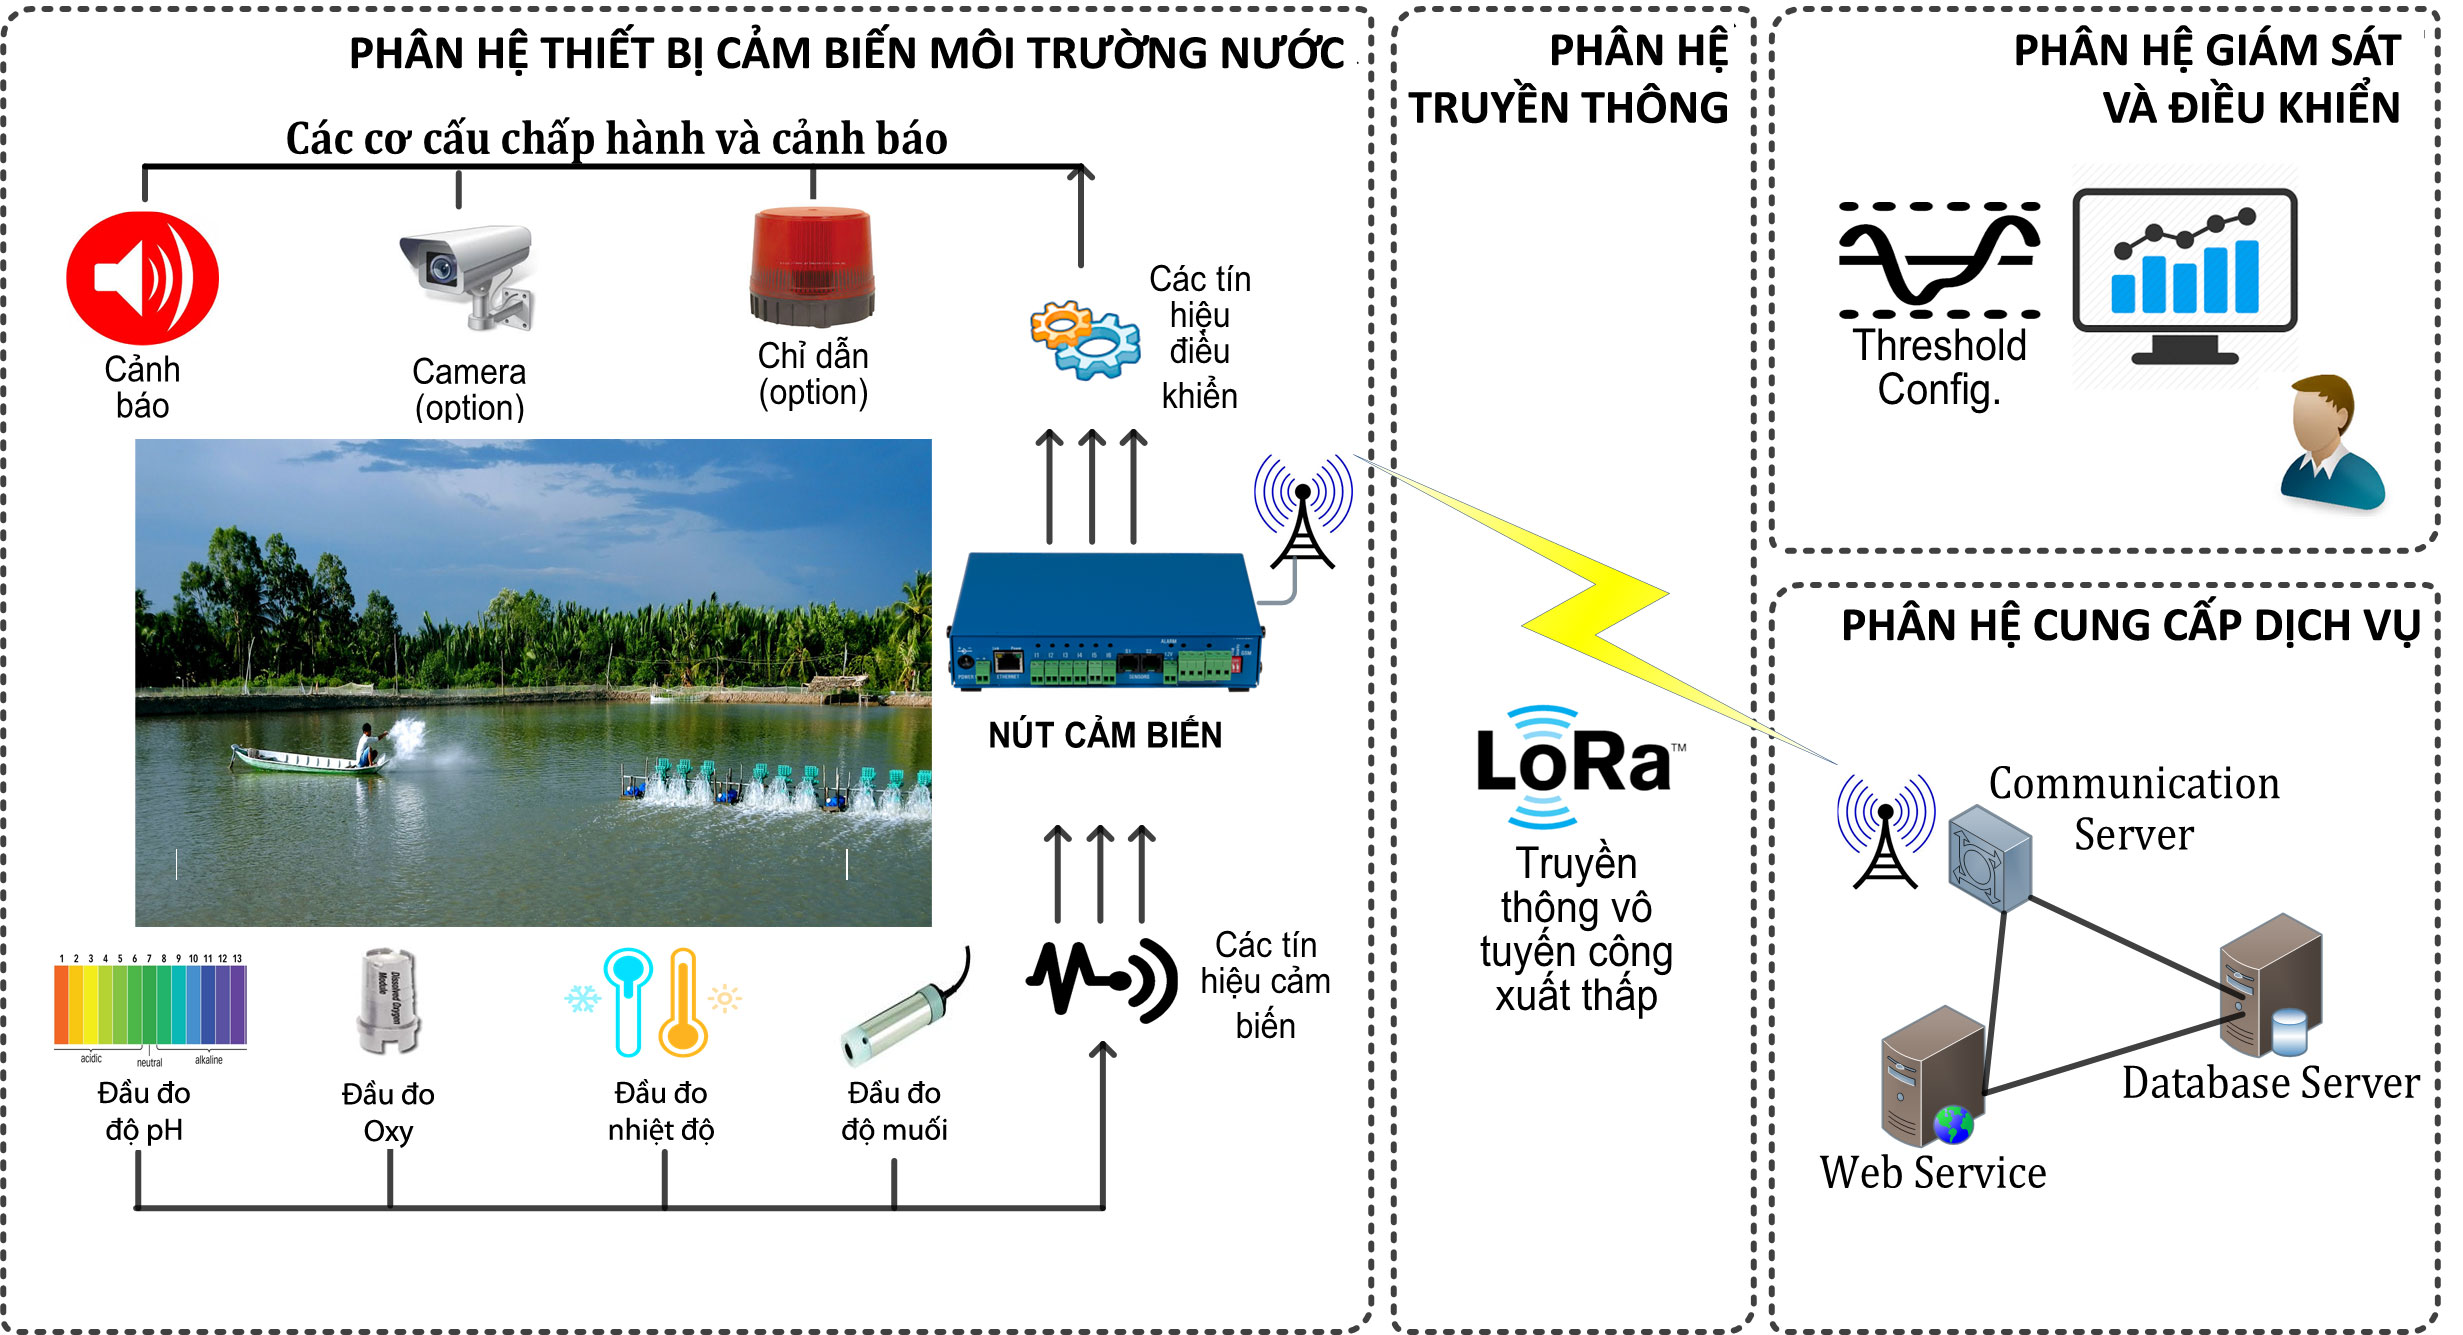
\includegraphics[scale=0.15]{image/kientrucLoRa}
\end{center}
\caption{Kiến trúc hệ thống}
\label{construction}
\end{figure}
\end{center}
\par Module LoRa SX1278 được lựa chọn để tích hợp vào thiết bị cảm biến như thể hiện trên Hình \ref{moduleSX1278}{}. Nút cảm biến được thiết kế và chế tạo tài phòng nghiên cứu SANSLAB, gồm các thành phần phần cứng chính như: phân hệ cảm biến các tham số môi trường nước, phân hệ truyền thông, phân hệ vi xử lý và điều khiển, phân hệ cấp nguồn và phân hệ hiển thị, cảnh tại chỗ. Phần mềm trên nút cảm biến gồm firmware và drivers điều khiển hoạt động các phân hệ và ngoại vi, thuật toán đa truy nhập cũng được nhúng trong firmware của thiết bị.
\subsection{Nút mạng cảm biến tích hợp module SX1278}
%\begin{center}
\begin{figure}[h]
	\begin{center}
		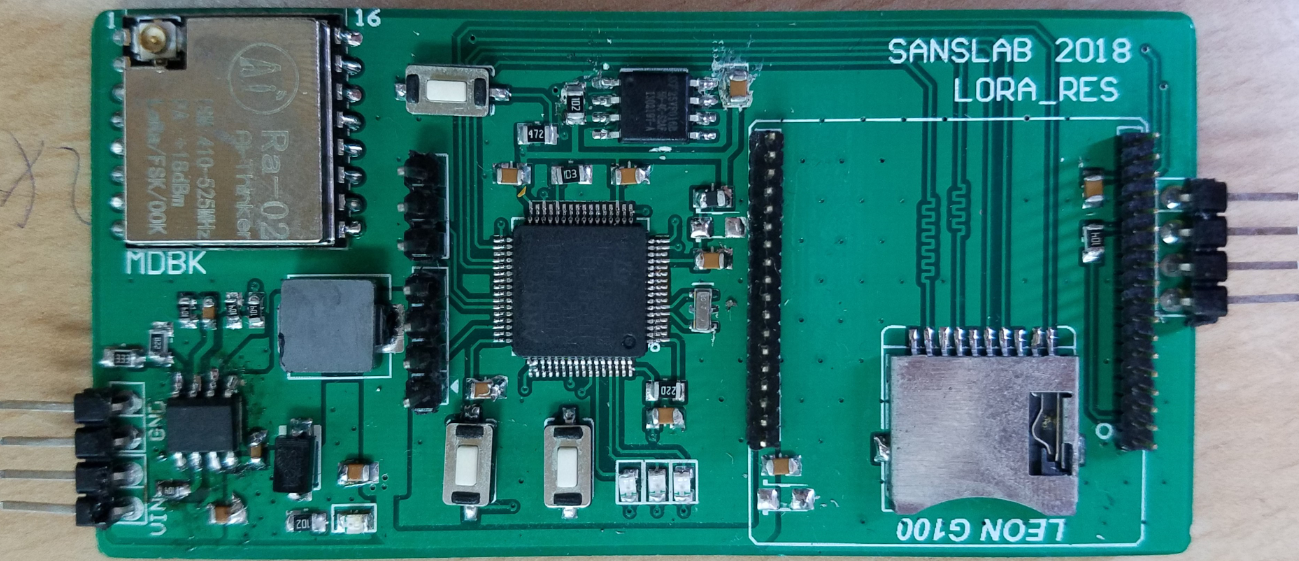
\includegraphics[scale=0.38]{image/hinh3_1}
	\end{center}
	\caption{Nút cảm biến tích hợp chip LoRa SX1278}
	\label{moduleSX1278}
\end{figure}
%\end{center}
\noindent Nút cảm biến được thiết kế gồm các khối có nhiệm vụ như sau:
\begin{itemize}
\item	Khối nguồn: có nhiệm vụ cung cấp nguồn cho toàn bộ mạch. Mức điện áp 3,3 V cung cấp cho vi điều khiển, thiết bị ngoại vi cùng với cảm biến. Nguồn cung cấp cho mạch là pin, nhỏ gọn và có thể sạc được nên rất phù hợp với các thiết bị trong mạng WSN,
\item	Khối xử lý trung tâm: có nhiệm vụ lấy dữ liệu từ các thiết bị cảm biến, xử lý rồi chuyển qua khối truyền thông, cũng như xử lý các thông tin nhận được từ khối truyền thông. Khối xử lý trung tâm sử dụng vi điều khiển STM32F1 là một loại vi điều khiển lõi Cortex M3 có tốc độ xử lý cao, cấu hình mạnh, tiết kiệm năng lượng với kích thước nhỏ gọn và giá thành rẻ,
\item	Khối truyền thông: có nhiệm vụ truyền nhận dữ liệu giữa các thiết bị trong mạng. Khối truyền thông sử dụng module LoRa Ai Thinker SX1278 được kết nối với khối xử lý trung tâm qua giao tiết SPI,
\item	Khối lưu trữ dữ liệu: được dùng để lưu trữ cấu hình hệ thống cùng với nhật ký cảm biến. Khối này gồm IC flash NAND SST25VF016B và thẻ nhớ. IC flash có tốc độ xử lý cao, dung lượng bộ nhớ nhỏ thích hợp với việc lưu trữ phần mềm cùng với cấu hình của hệ thống. Thẻ nhớ được sử dụng để lưu trữ nhật ký cảm biến, dễ dàng cho người sử dụng có thể kiểm tra và sao lưu dữ liêu.
\end{itemize}
\subsection{Mô hình hoạt động của hệ thống BKRES-LoRa}
Thuật toán đa truy nhập đề xuất được phát triển và thử nghiệm trên mô hình gồm 3 nút cảm biến và một Gateway như Hình \ref{normal}{}. Để đánh giá khả năng truyền dữ liệu, độ ổn định, khả năng tùy biến và tự cấu hình của các nút trong mạng, các thông số cơ bản của các nút sẽ được thiết lập theo như Bảng \ref{bang3_1}{}.
\begin{table}[h]
	\tabcolsep = 2cm
    \centering
    \caption{Bảng thông số cấu hình của các nút trong mạng}
    \begin{tabular}{|c|c|}
     	\hline
     	Thông số & Giá trị  \\
     	\hline
     	Channel & 11 (433 MHz)\\
     	\hline
     	BW & 125 kHz\\
     	\hline
     	CR & 4/5\\
     	\hline
     	SF & 7\\
     	\hline
     	Header & ON\\
     	\hline
     	CRC & ON\\
     	\hline
    \end{tabular}
    \label{bang3_1}
\end{table}
\par 
Hoạt động của mô hình được mô tả như sau. Ban đầu, mỗi nút mới (sau khi tự động cấu hình) sẽ gửi yêu cầu tham gia mạng đến Gateway, sau khi được chấp nhận thì nút bắt đầu quá trình gửi dữ liệu đến Gateway. Trong quá trình này, mỗi nút sẽ nhận dữ liệu đã được xử lý từ vi điều khiển, rồi gửi dữ liệu đến Gateway theo một chu kỳ định sẵn. Trong trường hợp xảy ra lỗi với bộ truyền thông LoRa, nút sẽ gửi dữ liệu trực tiếp đến server trung tâm qua mạng GSM (có sẵn trong BKRES phiên bản cũ), đến khi hết xảy ra lỗi với bộ truyền thông, nút lại bắt đầu lại quá trình như bình thường.\\
\begin{figure}[h]
	\centering
		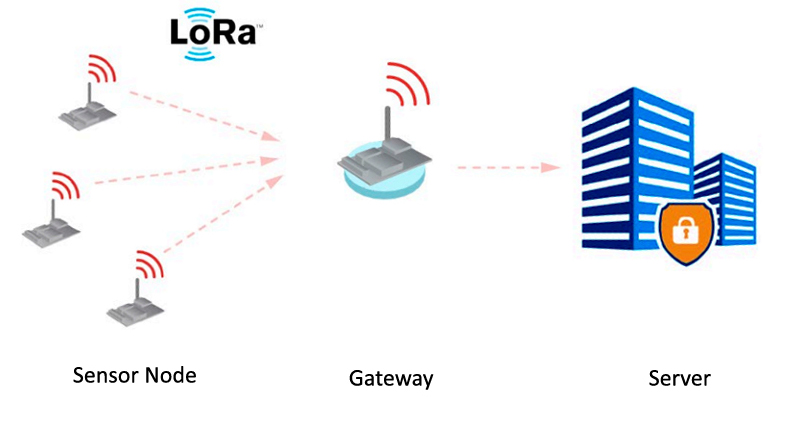
\includegraphics[scale=0.4]{image/normal}
	\caption{Mô hình hoạt động của mạng}
	\label{normal}
\end{figure}
\section{Xây dựng thuật toán đa truy nhập}
Do số lượng nút trong mạng ít, nên em quyết định sử dụng phương pháp đa truy nhập ngẫu nhiên, tức là khi nút có dữ liệu nó sẽ gửi luôn bản tin cho Gateway.
\subsection{Thuật toán đa truy nhập của Gateway}
Trong thuật toán đa truy nhập, Gateway có các nhiệm vụ chính sau:
 \begin{itemize}
 \item	Nhận dữ liệu từ các nút,
 \item	Quản lý nút trong mạng.
 \end{itemize}
 \par 
Sau khi đã tự cấu hình, trong vòng lặp vô hạn, Gateway liên tục mở kênh truyền để nhận bản tin. Nếu bản tin đó là do một nút mới gửi đến (nút chưa tham gia vào mạng) thì gateway sẽ tiến hành quá trình xác thực nút, rồi gửi bản tin phản hồi cho nút. Còn nếu bản tin là bản tin chứa dữ liệu, Gateway sẽ nhận và xử lý dữ liệu và tiếp tục quá trình mở kênh truyền để nhận dữ liệu. Algorithm \ref{gateway} thể hiện thuật toán xử lý của Gateway.
\begin{center}
\begin{algorithm}[h]
	\caption{Thuật toán của Gateway}
	\label{gateway}
	\begin{algorithmic}[1]
		\State $pass \gets @Rsanslab$
		\State Gateway tự động cấu hình  \Comment{Gateway sẽ tự động cài một số thông số như ID, SF, CR, tần số,...}
		\While{1}
			\If{Nhận được gói tin}
				\State $packet \gets packet\_receive$	\Comment{gói tin nhận được}
				\If{$packet$ là gói tin gửi dữ liệu}
					\State $data \gets packet.data$
					\State Xử lý dữ liệu	\Comment{Gateway có thể gửi dữ liệu lên Server, hiển thị hoặc lưu dữ liệu}
				\ElsIf{$packet$ là gói tin yêu cầu tham gia mạng}
					\State	$ID \gets packet.src$	\Comment{Lấy ID của nút gửi đến}
					\State	$authentication \gets packet.data$ \Comment{Lấy dữ liệu bản tin xác thực}
					\State 	$response \gets true$
					\If{$authentication \neq pass$ }
						\State $response \gets flase$
					\EndIf
					\State gửi bản tin phản hồi response cho nút ID
				\EndIf
			\EndIf		
		\EndWhile
	\end{algorithmic}
\end{algorithm}
\end{center}
\subsection{Thuật toán đa truy nhập của nút} 
Chức năng chính của nút trong thuật toán đa truy nhập:
\begin{itemize}
\item	Khi nút chưa tham gia mạng, nút sẽ gửi yêu cầu để tham gia mạng. Khi đó xảy ra một số trường hợp sau:
	\begin{itemize}
	\item	Quá trình yêu cầu không thành công, nút sẽ gửi lại,
	\item	Nếu bản tin xác thực sai, nút sẽ không hoạt động nữa,
	\item	Nếu quá trình yêu cầu tham gia mạng thành công, nút sẽ gửi dữ liệu.
	\end{itemize}
\item	Sau khi tham gia mạng thành công, nút sẽ gửi dữ liệu theo chu kỳ.
\end{itemize}
\begin{algorithm}[H]
	\caption{Thuật toán của Nút}
	\label{node}
	\begin{algorithmic}[1]
		\State {$msgAuthentication \gets @Rsanslab$}
		\State Nút tự động cấu hình  \Comment{Nút sẽ tự động cài một số thông số như ID, SF, CR, tần số,...}
		
		\State {$idGateway \gets$ Địa chỉ Gateway}		
		\State {$response \gets 2 $} \Comment{response = 0 --> bản tin xác thực chính xác; response = 1 --> bản tin xác thực không chính xác; response = 2 --> nút chưa tham gia mạng.}
		
		\State $RequestJoinNetworks(idGateway, msgAuthentication)$
		
		\While{1}
			\If{$response == 0$}
				\State $data \gets$ lấy dữ liệu từ cảm biến
				\State $cnt = 0$
				\Repeat
					\State $state \gets sendPacket(idGateway, data)$ 
					\If{$state > 0$} 
						\State $Delay()$
					\EndIf
					\State $cnt \gets cnt + 1$
				\Until{$state > 0$ and $cnt < threshold$} \Comment{threshold là số lần gửi tối đa}
			\ElsIf{$response == 1$} 
				\State $Sleep()$ 
				\Else
					\State $RequestJoinNetworks(idGateway, msgAuthentication)$
				\EndIf
			%\EndIf
		\EndWhile
	\end{algorithmic}
\end{algorithm}
Sau khi được cấu hình, nút sẽ gửi bản tin xác thực cho Gateway (ID của Gateway được thiết lập sẵn). Nút sẽ thực hiện quá trình yêu cầu tham gia mạng (quá trình yêu cầu tham gia mạng được mô tả bởi Algorithm \ref{RequestJoinNetworks}) đến khi thành công (nếu bản tin xác thực sai, nút sẽ dừng lại). Sau khi nút nhận được bản tin chấp nhận tham gia vào mạng của Gateway, nút sẽ tiến hành quá trình gửi dữ liệu. Quá trình xử lý của nút được thể hiện bởi Algorithm \ref{node}{}.
\par 
Trong quá trình yêu cầu tham gia vào mạng, nút sẽ gửi bản tin xác thực đến khi nào nhận lại được bản tin phản hồi của Gateway. Khi đó nút sẽ biết đươc mình đã được chấp thuận tham gia mạng hay chưa. Còn về phần Gateway, sau khi nhận được bản tin xác thực được gửi từ nút, Gateway sẽ kiểm tra bản tin xác thực đó có chính xác không. Kết quả của quá trình kiểm tra bản tin xác thực sẽ được Gateway gửi lại cho nút.
\begin{algorithm}[H]
\caption{RequestJoinNetworks}
\label{RequestJoinNetworks}
\begin{algorithmic}[1]
  \Procedure {RequestJoinNetworks}{$idGateway$, $msgAuthentication$}
	\Repeat
			\State $state \gets sendPacket(idGateway, msgAuthentication)$ 
			\Comment{state là trạng thái của quá trình gửi tin; state = 0 gửi bản tin thành công; state > 0 gửi bản tin chưa thành công}
			\If{$state > 0$} 
				\State Delay()
			\ElsIf{Nhận được bản tin hồi đáp từ Gateway}
				\State $response \gets packet\_receive.data$
				\If{$response$ không chính xác} 
					\State $state \gets 1$
				\EndIf
			\EndIf
	\Until{$state > 0$}
  \EndProcedure
\end{algorithmic}
\end{algorithm}
\section{Xây dựng chi tiết và đánh giá}
\subsection{Bản tin yêu cầu tham gia mạng}
Bản tin yêu cầu tham gia mạng sẽ được gửi khi nút đã tự cấu hình. Để giảm số lượng bản tin phải trao đổi giữa nút và Gateway để tham gia mạng, thì bản tin yêu cầu tham gia mạng sẽ chứa luôn bản tin xác thực. Trong quá trình thử nghiệm, chuỗi xác thực sẽ là "@Rsanslab" và được cấu hình sẵn trong firmware của cả nút và Gateway. Gateway sau khi nhận được bản tin yêu cầu tham gia mạng của nút, sẽ tách phần dữ liệu (chứa chuỗi xác thực) để so sánh với chuỗi xác thực của nó rồi tiến hành phản hồi cho nút. Cấu trúc gói yêu cầu tham gia mạng được mô tả trong bảng \ref{construction_rq}{}.
\begin{table}[h]
 \centering
    \caption{Cấu trúc bản tin yêu cầu tham gia mạng}
    \begin{tabular}{|c|c|}
    	\hline
     	Header & Data \\
     	\hline
     	2 byte & max. 255 byte\\
     	\hline
    \end{tabular}
    \label{construction_rq}
\end{table}
Trong thí nghiệm, bản tin yêu cầu tham gia mạng tương đối đơn giản mục đích để giảm thời gian xác thực của Gateway. Cấu trúc cụ thể bản tin:
\begin{itemize}
\item	Header: @R,
\item	Data: sanslab.
\end{itemize}
\par 
Luồng trao đổi bản tin giữa nút và Gateway sẽ được mô tả trong Hình \ref{refluong1}{}. Dữ liệu của bản tin phản hồi chỉ là "1" nếu bản tin xác thực chính xác hoặc là "0" nếu bản tin xác thực không chính xác.\\
\begin{figure}[h]
\begin{center}
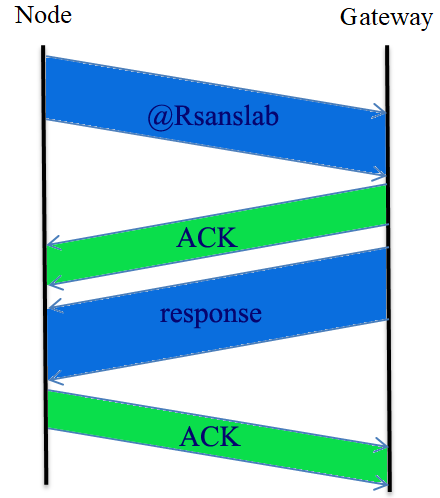
\includegraphics[scale= 0.5]{image/luong1}
\end{center}
\caption{Luồng trao đổi dữ liệu trong quá trình yêu cầu tham gia mạng}
\label{refluong1}
\end{figure}
\par 
Thuật toán yêu cầu tham gia mạng sẽ xảy ra 2 trường hợp:
\begin{itemize}
\item Trường hợp tốt nhất: Nút gửi yêu cầu tham gia mạng đến Gateway và nhận luôn được bản tin phải hồi của Gateway. Khi đó độ phức tạp của thuật toán là O(c).
\item Trường hợp xấu nhất: Nút gửi yêu cầu tham gia mạng đến Gateway nhưng không nhận được bản tin phản hồi của Gateway (hoặc gửi bản tin không thành công), nút sẽ gửi lại bản tin yêu cầu tham gia mạng. Khi đó độ phức tạp của thuật toán là O(n).
\end{itemize}
\subsection{Bản tin gửi dữ liệu}
Sau khi đã tham gia mạng thành công, theo chu kỳ, nút bắt đầu gửi bản tin chứa dữ liệu đến Gateway. Do số lượng nút nhỏ (3 đến 4 nút) nên khả năng xảy ra va chạm dẫn đến mất gói là rất ít. Do đó, nguyên nhân chính khiến nút gửi bản tin không thành công là do nút gửi bản tin không đúng vào thời điểm Gateway mở kênh truyền để nhận bản tin. Khi không gửi được bản tin thì nút sẽ trễ một khoảng thời gian, sau đó sẽ gửi lại bản tin. Cũng như bản tin yêu cầu tham gia mạng, bản tin chứa dữ liệu có phần header để nhận diện, ngoài ra bản tin còn chứa các thông số khác. Bản \ref{construction_data} mô tả cấu trúc bản tin gửi dữ liệu.\\
\begin{table}[h]
\centering
\caption{Cấu trúc bản tin dữ liệu}
	\begin{tabular}{|c|c|c|c|c|c|}
	\hline
	Header & IMEI & Command\_ID & Timestamp & Data & End \\
	\hline
	7 byte & 15 byte & 1 byte & 7 byte & max. 255 byte & 2 byte\\
	\hline 
	\end{tabular}
	\label{construction_data}
\end{table}\\
Luồng trao đổi bản tin dữ nút và Gateway được mô tả trong Hình \ref{senddata}{}.
\begin{figure}[htp]
\label{senddata}
\subfigure[Gửi bản tin thành công.]
  {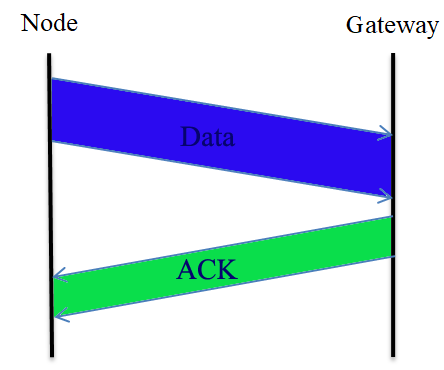
\includegraphics[width = .49\linewidth]{image/send_data}}\hfill
\subfigure[Gửi bản tin gặp xung đột và gửi lại.]
  {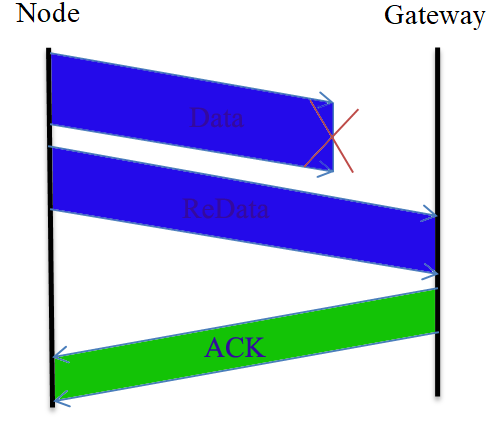
\includegraphics[width = .49\linewidth]{image/resend_data}}
  \caption{Luồng dữ liệu trong hai trường hợp}
\end{figure}
\begin{itemize}
\item Header: chứa dấu hiệu nhận diện bản tin chứa dữ liệu ("@DN") và kích thước của bản tin,
\item IMEI: là mã nhận dạng giữa các thiết bị với nhau, mỗi thiết bị có một IMEI khác nhau được cấu hình sẵn,
\item Command\_ID: là loại bản tin,
\item Timestamp: chứa thông tin về thời gian của dữ liệu (gồm: ngày, tháng, năm, giờ, phút, giây) được lấy từ vi điều khiển,
\item Data: chứa dữ liệu các thông số môi trường nước, gồm lần lượt các trường sau: pH, Oxy, Salt, Temp, $NH_3$, $H_2S$, $NO_2$,
\item End: báo hiệu kết thúc bản tin, là ký tự "\$".
\end{itemize}
Trong cả hai trường hợp gửi bản tin gặp xung đột và không gặp xung đột độ phức tạp của thuật toán là O(c) do số lần gửi lại của nút không được quá số lần quy định để đảm bảo tính thời gian thực của dữ liệu.
\section{Kết luận}
Sau khi đã xây dựng và đánh giá thuật toán đa truy nhập một cách kỹ lưỡng, thuật toán sẽ được triển khai dưới dạng code và nhúng vào những thiết bị trong hệ thống BKRES-LoRa. Quá trình thử nghiệm cùng với kết quả thử nghiệm sẽ được mô tả trong Chương \ref{chapter4}{}.



